\documentclass[
    11pt, % Set the default font size, options include: 8pt, 9pt, 10pt, 11pt, 12pt, 14pt, 17pt, 20pt
    %
    aspectratio=169, % Uncomment to set the aspect ratio to a 16:9 ratio which matches the aspect ratio of 1080p and 4K screens and projectors
    handout
]{beamer}

%\graphicspath{{Images/}{./}} % Specifies where to look for included images (trailing slash required)
\usepackage{booktabs} % Allows the use of \toprule, \midrule and \bottomrule for better rules in tables

%\usepackage{appendixnumberbeamer} %If you want a separate slide counter for your appendix



%%% To add citations
%\usepackage{biblatex}



%%% Customize Theme %%%%%%%%%%%%%%%%%%%%%%
\usetheme{Madrid} % You can use other themes too, but this changes many things. I've found Madrid to be the best for this color scheme

%fg = font color
%bg = background color

% ! WARNING ! : Many colors are linked to multiple attributes, so changing one color can have unexpected changes!

% If you want to tweak the shading of orange and red, tweak the below 2 lines:
\definecolor{myRed}{RGB}{134,31,65}
\definecolor{myOrange}{RGB}{229, 117, 31}

% Bottom right hand color
\setbeamercolor*{structure}{bg=myRed!20,fg=myRed!90}

\setbeamercolor*{palette primary}{use=structure,fg=white,bg=structure.fg} %?
\setbeamercolor*{palette secondary}{use=structure,fg=myRed,bg=white}
    %bottom left of footer & bar between title & top bubbles
\setbeamercolor*{palette tertiary}{use=structure,fg=white,bg=myRed} 

\setbeamercolor{frametitle}{bg=myRed!85,fg=white} %title of each slide

\setbeamercolor*{titlelike}{parent=palette primary} %?
%\setbeamercolor{titlelike}{parent=palette primary,fg=structure.fg!50!myRed}

%for miniframe (very top) AND center footer
\setbeamercolor{section in head/foot}{fg=myOrange, bg=white}

%%% Specific Colors %%%
\setbeamercolor{item projected}{bg=myOrange}
\setbeamertemplate{enumerate items}{bg=myOrange}

\setbeamercolor{itemize item}{fg=myOrange}
\setbeamercolor{itemize subitem}{fg=myOrange}

\setbeamercolor{button}{bg=myOrange}

%%% Edits ONLY the TOC slide %%%
\setbeamercolor{section in toc}{fg=black}
\setbeamercolor{subsection in toc}{fg=black}

%%% Block Colors %%%
% Standard block %
    \setbeamercolor{block title}{bg=myOrange, fg=white}
    \setbeamercolor{block body}{bg=myOrange!20}

% Alerted block % If you want to customize it's color
    %\setbeamercolor{block title alerted}{bg=cyan, fg=white}
    %\setbeamercolor{block body alerted}{bg=cyan!10}

% Example block % If you want to customize it's color
    %\setbeamercolor{block title example}{bg=cyan, fg=white}
    %\setbeamercolor{block body example}{bg=cyan!10}

%---------------------------------------------------------
%	SELECT FONT THEME & FONTS
%---------------------------------------------------------
\usefonttheme{default} % Typeset using the default sans serif font
\usepackage{palatino} % Use the Palatino font for serif text
\usepackage[default]{opensans} % Use the Open Sans font for sans serif text
\useinnertheme{circles}

%---------------------------------------------------------
%	SELECT OUTER THEME
%---------------------------------------------------------
% Outer themes change the overall layout of slides, such as: header and footer lines, sidebars and slide titles. Uncomment each theme in turn to see what changes it makes to your presentation.

\useoutertheme{default}
%\useoutertheme{miniframes}

%\useoutertheme{infolines}
%\useoutertheme{smoothbars}
%\useoutertheme{sidebar}
%\useoutertheme{split}
%\useoutertheme{shadow}
%\useoutertheme{tree}
%\useoutertheme{smoothtree}

%---------------------------------------------------------
%	PRESENTATION INFORMATION
%---------------------------------------------------------


\usepackage{listings}
\usepackage{amssymb}
\usepackage{pifont}% http://ctan.org/pkg/pifont
\newcommand{\cmark}{\ding{51}}%
\newcommand{\xmark}{\ding{55}}%
\usepackage{subcaption}

\usepackage{graphicx}
\graphicspath{ {./images/} }

\usepackage{hyperref}
\hypersetup{
    colorlinks=true,
    linkcolor=blue,
    filecolor=magenta,      
    urlcolor=cyan,
    pdftitle={Overleaf Example},
    pdfpagemode=FullScreen,
    }

\usepackage{mathrsfs}
\usepackage{tikz} 
%\usetikzlibrary{shapes.geometric, fit}

\title[A Measure for (weak) convexity]{MA-INF 4306 Lab Development and Application of Data Mining and
Learning Systems: Big Data \\ A measure for (weak) convexity}
\subtitle{Final Presentation}
\author[Timon Oerder]{Author: Timon Oerder, Mat.-Nr. 2679722}

\institute[]{Institut für Informatik Uni Bonn \\ \smallskip \textit{s6tioerd@uni-bonn.de}}

\date[\today]

\logo{\scalebox{0.3}{\includegraphics[width=0.15\textwidth]{logo}\hspace{0.1cm}\includegraphics[width=0.145\textwidth]{institutelogo}\par\vspace{1cm}}}


%---------------------------------------------------------
%---------------------------------------------------------
%---------------------------------------------------------
\begin{document}

%---------------------------------------------------------
%	TITLE SLIDE
%---------------------------------------------------------
\section{}
\begin{frame}
	\titlepage % Output the title slide, automatically created using the text entered in the PRESENTATION INFORMATION block above
 
\end{frame}

%---------------------------------------------------------
%	TABLE OF CONTENTS SLIDE
%---------------------------------------------------------
% References sections and subsections, specified with the standard \section and \subsection commands. If you want to display all sections and subsections on one slide, just use \tableofcontents. If you want to just display each section one at a time (in subsequent slides) use \tableofcontents[pausesections].

\begin{frame}
	\frametitle{Table of contents} % Slide title, remove this command for no title
	
	\tableofcontents % Output the table of contents (all sections on one slide)
	%\tableofcontents[pausesections] % Output the table of contents (break sections up across separate slides)
\end{frame}


%---------------------------------------------------------
%	PRESENTATION BODY SLIDES
%---------------------------------------------------------
\section{The top-level roadmap} % Note all sections and subsections are automatically placed in your table of contents
\begin{frame}
\frametitle{The top-level road-map}
\begin{enumerate}
\item<1-> Define a measure for (weak) convexity
\item<2-> Test that measure on artificial data
\item<3-> Test the measure on real-world data
\end{enumerate}
\end{frame}

\section{Questions addressed since the last meeting}
\begin{frame}
\frametitle{Questions addressed since the last meeting}
\begin{enumerate}
\item<1-> Sanity check for the convex hull Algorithm
\item<2-> Can $\epsilon$ and $\theta$ be modified as a measure?
\item<3-> Idea for measures.
\end{enumerate}
\end{frame}

\section{Sanity check for the convex hull Algorithm}
\begin{frame}
\frametitle{Sanity check for the convex hull Algorithm}
\begin{figure}
\centering
\begin{subfigure}{0.3\textwidth}
    \includegraphics[width=\textwidth]{testcase-grid}
    \caption{Testcase grid}
    \label{fig:first}
\end{subfigure}
\hfill
\begin{subfigure}{0.3\textwidth}
    \includegraphics[width=\textwidth]{testcase-line}
    \caption{Testcase line}
    \label{fig:second}
\end{subfigure}
\caption{Application with $\theta=3$, $\epsilon=0.0$ and step distance; \\ class 0 is red; class 1 is blue; class 1 assigned as the convex hull of class 0 is orange}
\end{figure}
\end{frame}

\section{Can $\epsilon$ and $\theta$ be modified as a measure?}
\begin{frame}
\frametitle{Can $\epsilon$ and $\theta$ be modified as a measure? (I)}
In theory we can combine the notion of ($\theta$, $\epsilon$)-convexity as follows:
$A \subset X, z \in X, \epsilon \geq 0, \theta \geq 0$. \\
$z \in A \Leftrightarrow \exists x,y \in A: d(x,z)+d(z,y) \textcolor{blue}{\leq d(x,y) + \epsilon} \land d(x,z)+d(z,y) \textcolor{blue}{\geq d(x,y) - \epsilon} \land \textcolor{red}{d(x,y) \leq \theta}$
\begin{enumerate}
\item<2-> For $\epsilon=0$ and $\theta \geq \underset{x,y \in A}{argmax}~ d(x,y)$ we get the standard notion for convexity. {\tiny ($z \in A \Leftrightarrow \exists x,y \in A: d(x,z)+d(z,y)=d(x,y)$)}
\item<3-> For $\epsilon=0$ and $\theta \in [0, ... \underset{x,y \in A}{argmax}~ d(x,y))$ we get $\theta$-convexity \cite{Lab2324BigData/Main}. {\tiny ($z \in A \Leftrightarrow \exists x,y \in A: d(x,z)+d(z,y)=d(x,y) \land \textcolor{red}{d(x,y) \leq \theta}$)}
\item<4-> $\epsilon$ "smears" the boundary of the convex hull. For a big enough $\epsilon$ every point $z \in X$ is contained in the convex hull.
\item<5-> If we find a "core" object $C \subset A$ which is the biggest convex subset, for what parameter $\epsilon$ and $\theta$ as inputs to a convex hull algorithm do we get $A$ as result? 
\end{enumerate}
\end{frame}

\begin{frame}
\frametitle{Can $\epsilon$ and $\theta$ be modified as a measure? (II)}
\begin{center}
{ How does the number of components and the number of vertices in the convex hull develop for different $\theta$s? }
\end{center}

\begin{figure}
\centering
\onslide<2->{
\begin{subfigure}{0.25\textwidth}
    \includegraphics[width=\textwidth]{thetaepsilon/theta0.1}
    \caption{$\theta=0.1$}
    \label{fig:first}
\end{subfigure}
}
\hfill
\onslide<3->{
\begin{subfigure}{0.25\textwidth}
    \includegraphics[width=\textwidth]{thetaepsilon/theta2.32}
    \caption{$\theta=2.32$}
    \label{fig:second}
\end{subfigure}
}
\hfill
\onslide<4->{
\begin{subfigure}{0.25\textwidth}
    \includegraphics[width=\textwidth]{thetaepsilon/theta4.54}
    \caption{$\theta=4.54$}
    \label{fig:second}
\end{subfigure}
}
\caption{Application of the Algorithm with different $\theta$, $\epsilon=0.0$,  $n=1000$ vertices, 4 clusters  and step distance; \\ class 0 is red; class 1 is blue; class 1 assigned as the convex hull of class 0 is orange}
\end{figure}
\end{frame}

\begin{frame}
\frametitle{Can $\epsilon$ and $\theta$ be modified as a measure? (III)}
\begin{figure}
\centering
\onslide<1->{
\begin{subfigure}{0.3\textwidth}
    \includegraphics[width=\textwidth]{thetaepsilon/theta0.1-cluster}
    \caption{$\theta=0.1$}
    \label{fig:first}
\end{subfigure}
}
\hfill
\onslide<1->{
\begin{subfigure}{0.3\textwidth}
    \includegraphics[width=\textwidth]{thetaepsilon/theta2.32-cluster}
    \caption{$\theta=2.32$}
    \label{fig:second}
\end{subfigure}
}
\hfill
\onslide<1->{
\begin{subfigure}{0.3\textwidth}
    \includegraphics[width=\textwidth]{thetaepsilon/theta4.54-cluster}
    \caption{$\theta=4.54$}
    \label{fig:second}
\end{subfigure}
}
\caption{Application of the Algorithm with different $\theta$, $\epsilon=0.0$,  $n=1000$ vertices, 4 clusters  and step distance; \\ vertices not part of a component and not part of the convex hull are grey, all other vertices are brown, blue or purple depending on their component.}
\end{figure}
\end{frame}

\begin{frame}
\frametitle{Can $\epsilon$ and $\theta$ be modified as a measure? (IV)}
\begin{figure}
\centering
\begin{subfigure}{0.4\textwidth}
    \includegraphics[width=\textwidth]{thetaepsilon/numberOfComponents}
    \caption{Number of Components}
    \label{fig:first}
\end{subfigure}
\hfill
\begin{subfigure}{0.4\textwidth}
    \includegraphics[width=\textwidth]{thetaepsilon/numberOfPoints}
    \caption{Number of Vertices in the convex hull}
    \label{fig:second}
\end{subfigure}
\caption{Application of the Algorithm with different $\theta$, $\epsilon=0.0$,  $n=1000$ vertices, 4 clusters  and step distance;}
\end{figure}
\onslide<2->{
No answers for now.
Questions for the future:
Does a core object exists? Is it unique?
}
\end{frame}
\section{Convexity Measure Proposal 1}
\begin{frame}
\frametitle{Convexity Measure Proposal 1 (I)}
We can calculate a measure for convexity by looking at all the shortest paths between nodes and see how often we need to take a vertex outside of our set on such a path. \par
\pause
For $x,y \in V: sp(x,y)=\{ \{k_1..k_n\} | \{k_1..k_n\} \text{are verticies on a shortest path from x to y} \}$. \newline
$A \subset V: C_1(A)=\underset{x,y \in A~}{\sum} ( \frac{1}{|sp(x,y)|} \cdot \underset{p \in sp(x,y)}{\sum} |p\setminus A| )$
\pause
\begin{center}
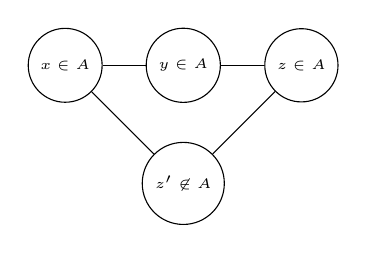
\begin{tikzpicture}[scale=0.5, node distance={15mm}, main/.style = {draw, circle}] 
\node[main] (1) {\tiny $x \in A$}; 
\node[main] (2) [right of=1] {\tiny $y  \in A$}; 
\node[main] (3) [right of=2] {\tiny $z \in A$}; 
\node[main] (4) [below of=2] {\tiny $z'  \not \in A$};
\draw (1) -- (2);
\draw (2) -- (3);
\draw (1) -- (4);
\draw (4) -- (3);
\end{tikzpicture}
\end{center}
\end{frame}

\begin{frame}
\frametitle{Convexity Measure Proposal 1 (II)}
\begin{center}
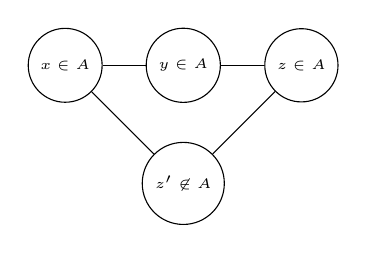
\begin{tikzpicture}[scale=0.5, node distance={15mm}, main/.style = {draw, circle}] 
\node[main] (1) {\tiny $x \in A$}; 
\node[main] (2) [right of=1] {\tiny $y  \in A$}; 
\node[main] (3) [right of=2] {\tiny $z \in A$}; 
\node[main] (4) [below of=2] {\tiny $z'  \not \in A$};
\draw (1) -- (2);
\draw (2) -- (3);
\draw (1) -- (4);
\draw (4) -- (3);
\end{tikzpicture}
\end{center}
\pause
$A=\{x,y,z\}$ ~~ $sp(x,y)=\{\{x,y\}\},~ sp(y,z)=\{\{y,z\}\},~ sp(x,z)=\{\{x,y,z\},\{x,y,z'\}\}$
\pause 
$C_1(A)= \frac{1}{|sp(x,y)|} \cdot \underset{p \in sp(x,y)}{\sum} |p\setminus A| + \frac{1}{|sp(y,z)|} \cdot \underset{p \in sp(y,z)}{\sum} |p\setminus A| + \frac{1}{|sp(x,z)|} \cdot \underset{p \in sp(x,z)}{\sum} |p\setminus A|$
\pause
$C_1(A)= \frac{1}{\underbrace{|\{\{x,y\}\}|}_{=1}} \cdot | \underbrace{\{x,y\} \setminus A}_{=\emptyset} | + \frac{1}{\underbrace{|\{\{y,z\}\}|}_{=1}} \cdot | \underbrace{\{y,z\} \setminus A}_{=\emptyset} | + \frac{1}{\underbrace{|\{\{x,y,z\},\{x,y,z'\}\}|}_{=2}} \cdot | \underbrace{\{x,y,z\} \setminus A}_{=\emptyset} | + \frac{1}{\underbrace{|\{\{x,y,z\},\{x,y,z'\}\}|}_{=2}} \cdot | \underbrace{\{x,y,z'\} \setminus A}_{=\{z'\}} | = \frac{1}{2}
$
\end{frame}

\section{Convexity Measure Proposal 2}
\begin{frame}
\frametitle{Convexity Measure Proposal 2 (I)}
\begin{block}{Polygonal Entropy: a convexity measure \cite{Lab2324BigData/PolygonalEntropy}}
How much of the polygon is visible from any point in it? \\ \pause 
In a convex polygon, every point can see every other point. \\
$\Rightarrow$ What is the information this point gains/has about the rest of the polygon?
\end{block}
\pause
Let $P$ be the set of all points of a polygon on it`s boundary and interior. \\
For a point $p \in P: V(p,P)$ defines the visible polygon as viewed from p and $A(V(p,P))$ the visible area. The area of the polygon will be denoted $A(P)$. \\ 
\pause
The sum of all visible areas for every point in the polygon:
$AT(P)=\underset{p \in P}{\int} A(V(p,P)) dp$ \\
\pause
Probability density function:
$f(p) = A(V(p,P))/AT(P)$ \\
\pause
Polygonal Entropy $ E(P) = -\underset{p \in P}{\int} f(p) ln (f(p)) dp$ \\
\pause
\textcolor{red}{Convexity of a polygon P is $C(P) = E(P) / E_{max}(P)$ with $E_{max}(P) = -ln(1/A(P))$}\\
\end{frame}

\begin{frame}
\frametitle{Convexity Measure Proposal 2 (II)}
We can adapt that definition to graphs $G=(V,E)$: \\
Let $p$ be a point in the set $P \subset V$. \\ \pause
For any $p \in P$ the Area of visible points of P in P is defined as $A(V_{in}(p,P))=|\{p' \in P | \textcolor{blue}{\exists path \in sp(p, p'): path \setminus P = \emptyset}\}|$, \\ \pause
the Area of visible points of P in V (in the convex hull) is defined as $A(V_{all}(p,P))=|\{p' \in P \}|$\\ \pause
$A(P)=|P|$ is analog defined as the cardinality of the set. \\ \pause
$AT(P)=\underset{p \in P}{\sum} A(V_{all}(p,P))$ \pause
$=\underset{p \in P}{\sum} |\{p' \in P \}| = |P| \cdot |P|$ \\ \pause
$f(p) = A(V_{in}(p,P))/AT(P) = \frac{A(V_{in}(p,P))}{|P|^2}$ \\ \pause
Entropy of a vertex set $ E(P) = -\underset{p \in P}{\sum} f(p) ln (f(p))$ \\
\pause
\textcolor{red}{Convexity of a set of vertices is $C_2(P) = E(P) / E_{max}(P)$ with $E_{max}(P) = -ln(1/A(P))$}\\
\end{frame}
\section{Testcases/First Results}
\begin{frame}
\frametitle{First Results (I)}
\begin{figure}
\centering
\begin{subfigure}{0.4\textwidth}
    \includegraphics[width=\textwidth]{testcasemeasures-1}
    \caption{$C_1(P)=0$, $C_2(P)=1$}
    \label{fig:first}
\end{subfigure}
\hfill
\begin{subfigure}{0.4\textwidth}
    \includegraphics[width=\textwidth]{testcasemeasures-2}
    \caption{$C_1(P) \approx 1.3$, $C_2(P) \approx 0.65$}
    \label{fig:second}
\end{subfigure}
\caption{Step distance}
\end{figure}
\end{frame}

\begin{frame}
\frametitle{First Results (II)}
\begin{figure}
\centering
\begin{subfigure}{0.4\textwidth}
    \includegraphics[width=\textwidth]{testcasemeasures-3}
    \caption{$\theta=2$, $C_1(P) \approx 1.090 $, $C_2(P) \approx 0.65$, convex}
    \label{fig:first}
\end{subfigure}
\hfill
\begin{subfigure}{0.4\textwidth}
    \includegraphics[width=\textwidth]{testcasemeasures-4}
    \caption{$\theta=3$, $C_1(P) = 0$, $C_2(P) = 1$}
    \label{fig:second}
\end{subfigure}
\caption{Step distance; Results for measures after application of the convex hull algorithm}
\end{figure}
\end{frame}

\section{Next steps}
\begin{frame}
\frametitle{Next steps}
\begin{itemize}
\onslide<1->\item Can $\epsilon$ and $\theta$ be modified as a measure?
\onslide<2->\item Can we find a unique core?
\onslide<3->\item Any other measures to test?
\onslide<4->\item How do the measures behave relate to the notion of weak convexity?
\onslide<5->\item Find repository data sets to test the measure(s) on
\onslide<6->\item Test the measure(s)
\end{itemize}
\onslide<7->{\begin{exampleblock}{Thank you for your attention!}
\centering 
What are your questions?
\end{exampleblock}}
\end{frame}

\section{References}
\begin{frame}
\frametitle{References}
\bibliographystyle{alpha}
\bibliography{refs} 
\end{frame}

\appendix
\section{Appendix}
\end{document} 